\documentclass[10pt,twocolumn,letterpaper]{article}

\def\code#1{\texttt{#1}}
\usepackage{natbib}
%% Language and font encodings
\usepackage[french]{babel}
\usepackage[utf8x]{inputenc}
\usepackage[T1]{fontenc}
\usepackage{float}

%% Sets page size and margins
\usepackage[a4paper,top=3cm,bottom=2cm,left=3cm,right=3cm,marginparwidth=1.75cm]{geometry}

%% Useful packages
\usepackage{amsmath}
\usepackage{graphicx}
\usepackage[colorinlistoftodos]{todonotes}
\usepackage[colorlinks=true, allcolors=blue]{hyperref}

\bibliographystyle{unsrt}
%% Title
\title{
		\usefont{OT1}{bch}{b}{n}
		\normalfont \normalsize \textsc{Mines ParisTech - Ms HPC-AI} \\ [10pt]
		\huge Projet de Programmation Parallèle \\
}
\selectlanguage{french}
\usepackage{authblk}
\author{Aymeric MILLAN}
\affil{Cours de Jean-Marc GRATIEN}
\date{20 décembre 2021}

\begin{document}

\maketitle

\begin{abstract}
Voici le document regroupant les benchmarks des programmes 
SparseMV MPI (produit matrice CSR avec un vecteur), 
DenseMV MPI 
et life of boids multi threadé.

Le but du projet est de s'approprier différents outils de parallélisation de code : MPI pour la mémoire distribuée, et OMP/TBB pour la mémoire partagée. 
En plus de ces outils, ce projet apporte une vision générale sur les méthodologies de développement sur des clusters de calculs tels que celui du CEMEF. 
J'ai pu découvrir de nouveaux concepts tels que les jobs (OAR ici), 
l'utilisation et la réservation des noeuds de calcul ou par exemple l'étude des logs des exécutions en batch. 
\end{abstract}

\section{Récupérer le code}
Le code est disponible sur le GitHub, branche \code{dev-aympab}. 
Le répertoire d'accès sur le cluster du CEMEF est \code{aymeric.millan/}, vous y trouverez le contenu du GitHub dans \code{git\_sophia/}.
Le code est déjà compilé sur le cluster, les exécutables sont disponibles dans le répertoire \code{bin/}.
Pour life-of-boids, conan est nécessaire à la compilation et ne peut donc pas être compilé sur le CEMEF. 
Le projet est fonctionnel sur une machine avec gcc, cmake et conan.

\section{Logique d'implémentation}

Vous trouverez quelques informations sur les méthodologies d'implémentations de chaque programme dans leurs parties respectives.
Pour le benchmarking, j'ai utilisé un script shell qui formate les données des logs OAR en fichiers csv à l'aide d'une suite de commande shell.
Ensuite, à l'aide de python et surtout de la librairie \code{pandas}, j'ai traité les données avant de les afficher sur ces graphes.
Les données brutes sont disponibles dans le répertoire \code{logs/} du projet.

\section{Produit Matrice Dense \& Vecteur}

L'implémentation du produit matrice dense et vecteur a été la plus simple à réaliser, autant pour les communications MPI que la logique.

Le graphique ci-dessous montre l'évolution du temps de calcul en fonction du nombre de processeurs, pour différentes tailles de matrices.
Les traits pointillés représentent le temps de calcul en séquentiel, les traits pleins représentent le temps de calcul du noeud MPI le plus lent.
Les couleurs correspondent entre les temps séquentiels et parallèles.

\begin{figure}[H]
  \centering
  \caption{Rapport de performance DenseMV}
  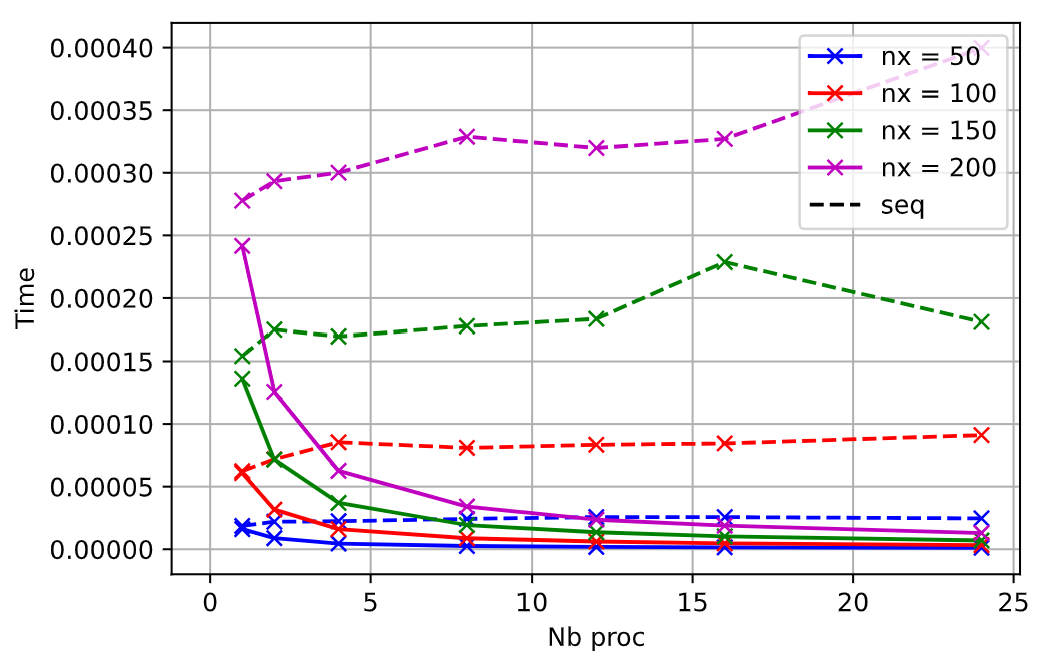
\includegraphics[width=0.49\textwidth]{figures/densemv_benchmark.png}
\end{figure}

Nous pouvons constater que, pour un noeud, les temps de calcul sont relativement similaires, 
mais dès que le nombre de noeuds augmente,le coût de calcul baisse drastiquement pour les matrices de grande taille.
Cela est moins vrai pour les matrices de petites tailles.

\section{Produit Matrice (CSR) \& Vecteur}

Pour le SpMV CSR, j'ai d'abord essayé d'utiliser un seul et même buffer pour envoyer les éléments
aux différents nodes. Ce n'était pas une bonne idée, car le programme ne fonctionnait pas avec des matrices de trop grandes tailles.
Le problème venait d'une commande \code{clear()} sur les \code{vector} contenant les buffers à envoyer.
Parfois, si la taille du buffer était trop grande, comme l'envoi était fait en asynchrone, le buffer avait le temps d'être \code{clear} avant d'être réellement envoyé.
Cette erreur était très compliquée à débugger car si les matrices étaient trop petites, l'envoi était fait quasi instantanément et tout fonctionnait bien.
Je suis donc parti sur du synchrone pour l'envoi des valeurs, de toute façon, pour un problème de cette taille, 
les communications sont bien trop couteuses et biaisent la durée de calcul.
C'est pourquoi elles ne sont pas prises en compte dans les benchmarks.

De plus, il est bon de noter que le découpage a été réalisé par lignes et non pas par valeurs. 
Bien entendu, cela n'est pas fidèle à la logique de la parallélisation MPI qui voudrait que les charges soient équilibrées pour chaque processus.
Cependant, comme nous résolvons un produit par une matrice Laplacienne, qui est tridiagonale, 
les charges seront équilibrées et nous n'avons pas à gérer les pondérations des valeurs entre deux processus si une ligne est coupée en deux.

\begin{figure}[H]
  \centering
  \caption{Rapport de performance SparseMV}
  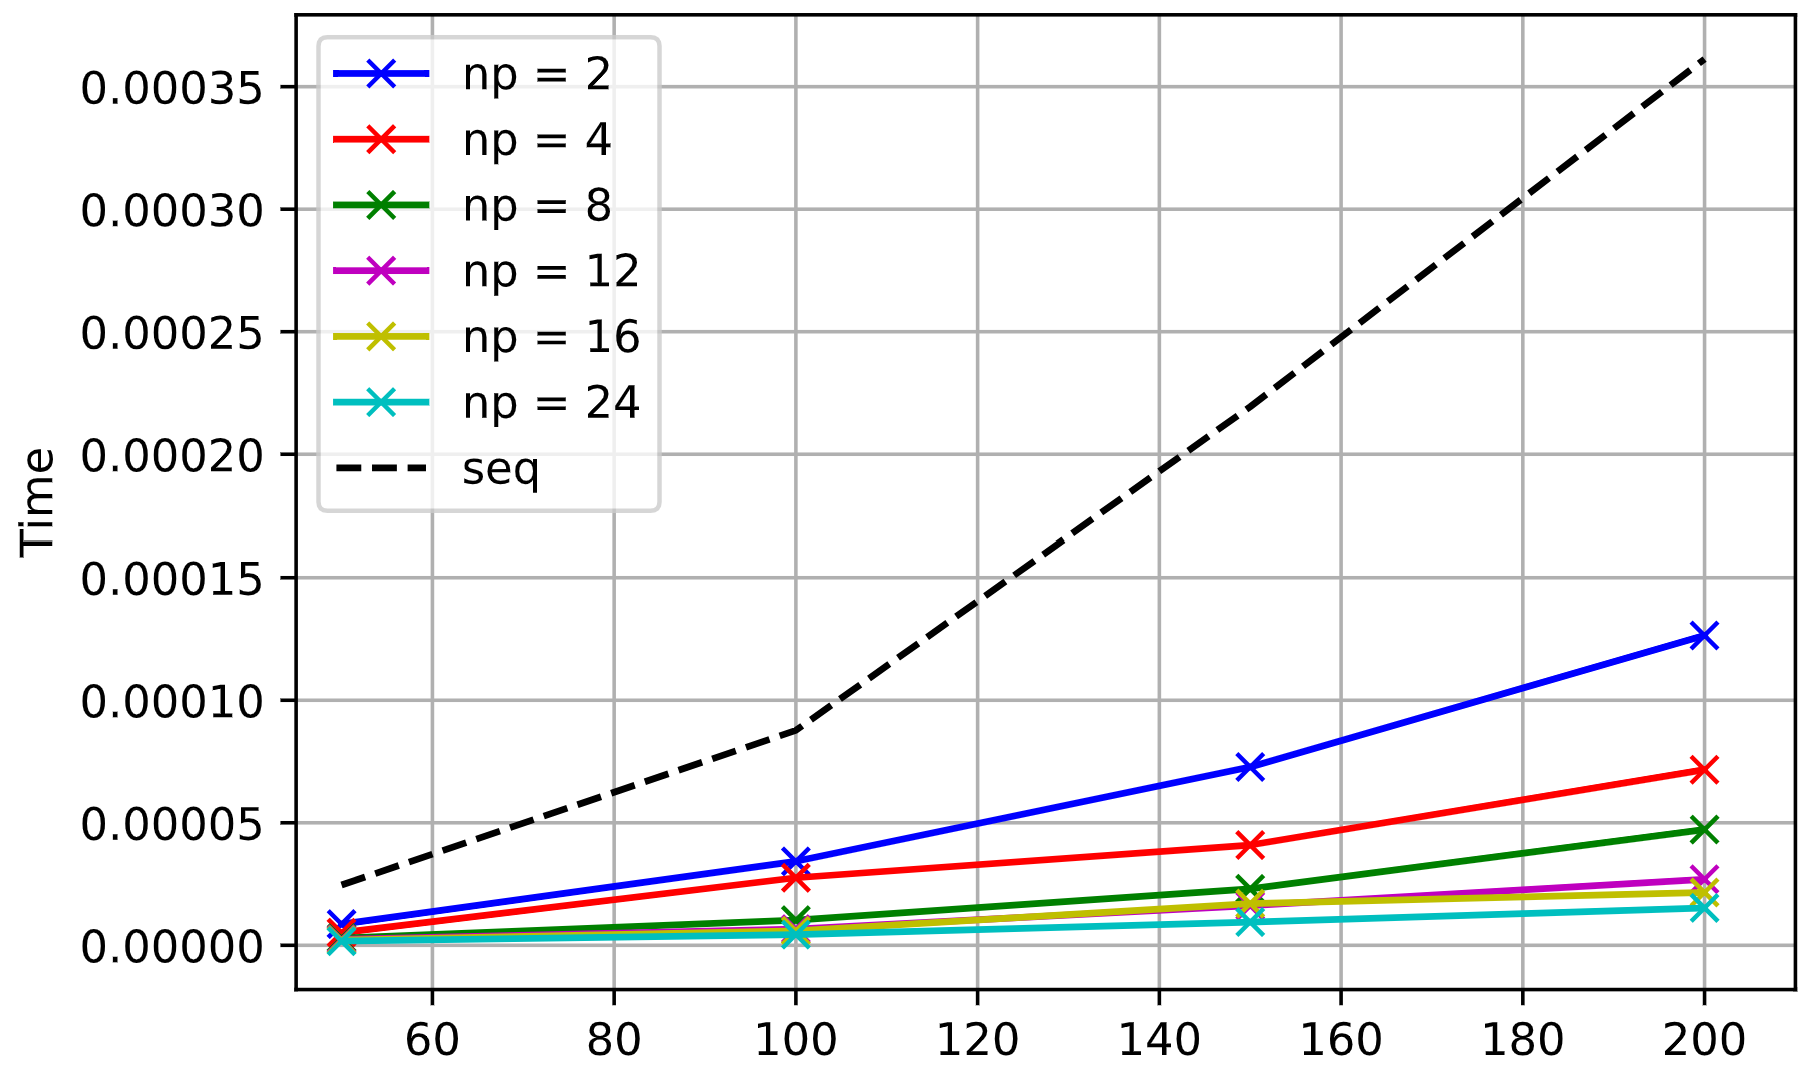
\includegraphics[width=0.49\textwidth]{figures/spmv_benchmark.png}
\end{figure}

Pour varier un peu, ce graphe affiche le temps de calcul en fonction de la taille de la matrice, pour
différents nombres de coeurs.
Les variables sont donc inversées par rapport au premier graphique. 
La courbe en pointillée correspond au temps de calcul séquentiel. 
On constate que le calcul SpMV est toujours plus rapide que celui de DenseMV avec MPI, et que le temps de calcul réduit drastiquement au début
(lorsqu'on passe de 1 a 2 nodes), puis ce temps de calcul réduit de moins en moins.

\section{Life-of-boids}

Pour l'application life-of-boids, j'ai isolé la boucle principale de calcul dans un exécutable \code{main\_profiling}, en retirant la partie graphique.
J'ai ensuite chronométré les exécutions d'un tour de boucle en fonction de la taille de départ du "flock".
Cela correspond au nombre d'agents dans notre système et ce paramètre est intrinsèquement lié au nombre de calculs effectués à chaque tour de boucle.

Les calculs ont été réalisés sur un \textbf{Intel Core i7-10870H CPU @ 2.20GHz}. Possédant \textbf{8 coeurs physiques, et 16 coeurs logiques} grâce à l'hyperthreading.

Ce premier graphique trace le temps d'éxecution en fonction de la taille de la population (flock) et du nombre de threads.
Les traits pointillés correspondent à l'éxecution avec OpenMP, les traits pleins à TBB. Enfin, le trait plein noir correspond à l'éxécution séquentielle.

\begin{figure}[H]
  \centering
  \caption{Flock of boids multithread}
  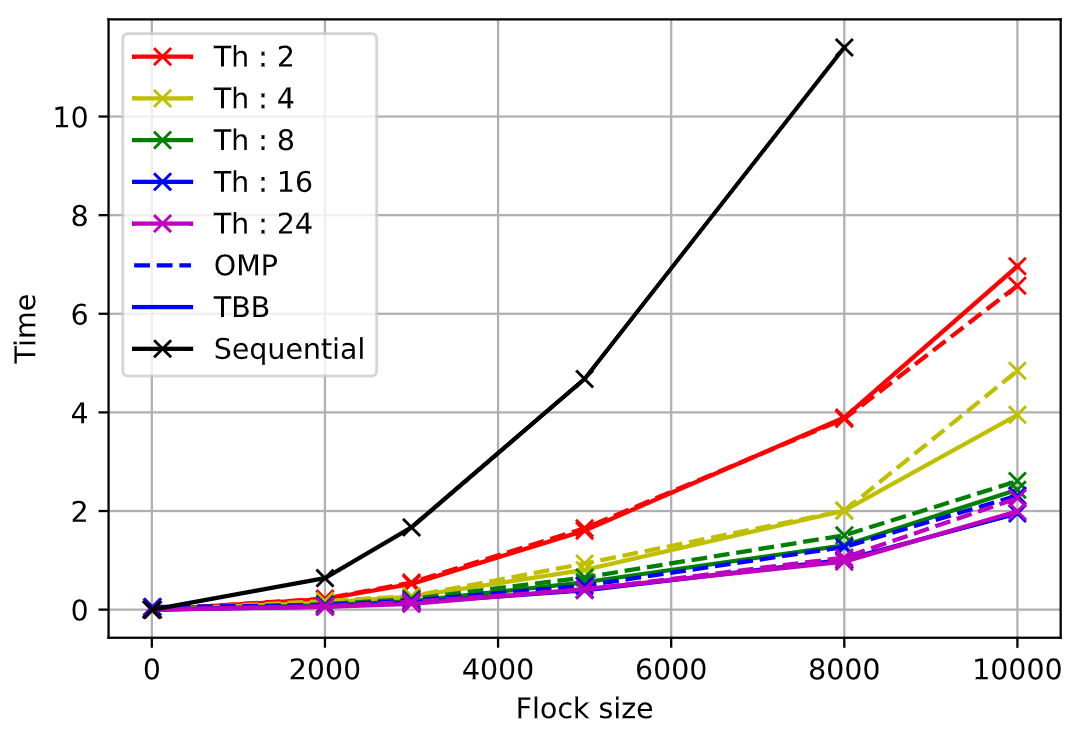
\includegraphics[width=0.49\textwidth]{figures/boids_with_seq.png}
\end{figure}

Nous pouvons constater que passer d'une exécution séquentielle à une éxecution parallèle avec ne serait-ce qu'avec 2 threads apporte un gain de performance considérable.

Cependant, intéressons nous à la performance des deux librairies, OMP et TBB, pour ceci, appuyons nous sur ce même graphique sans la version séquentielle.
On éxécute 100 tours de boucle cette fois : la finalité des calculs est de l'affichage graphique, donc ils vont être réalisés un grand nombre de fois à la suite.
C'est ce que nous essayons de simuler ici.

\begin{figure}[H]
  \centering
  \caption{Comparaison OMP et TBB sur 100 tour de boucle}
  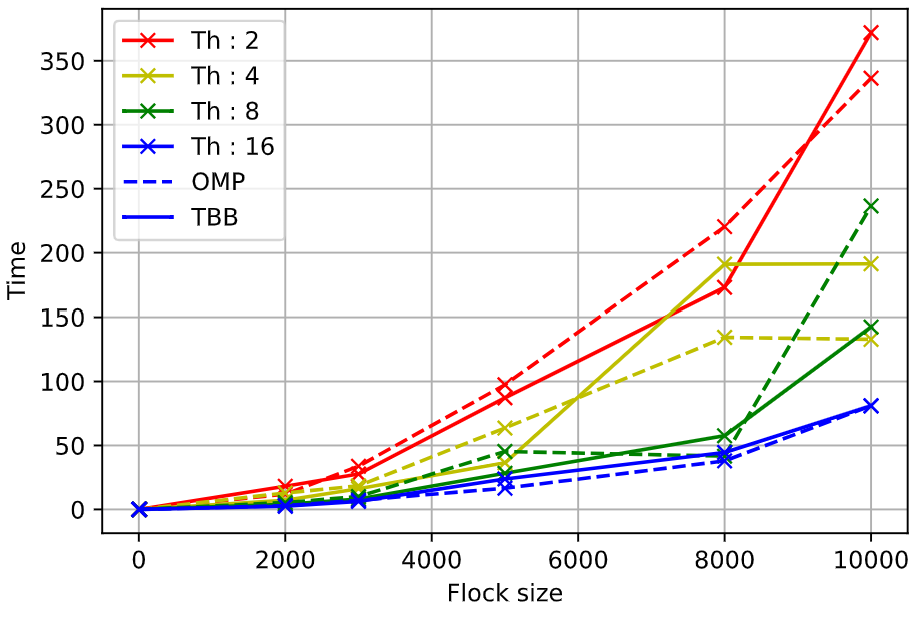
\includegraphics[width=0.49\textwidth]{figures/boids_100_exec.png}
\end{figure}

Ce graphique nous montre que, sur cette machine et ce processeur, TBB semble être légèrement meilleur que OMP.
Lorsqu'on passe de 2 à 4 threads ou de 4 à 8, la durée d'exécution tend à être divisé par deux.
Cela parait logique car la machine possède 8 coeurs.
Sur 100 exécutions, l'hyperthreading semble avoir plus d'impact, le gain de performance entre 8 et 16 threads reste intéressant.
Comme nous l'avons vu sur le graphique précédent, au delà d'un certain seuil, augmenter le nombre de threads n'est pas utile.

\section*{Conclusions}
\textbf{Mémoire distribuée : }sans surprise, plus le nombre de processus augmente, plus le calcul sur chaque processus est rapide.
Cependant, il est bon de noter que pour un problème de cette taille, les communications prennent un temps trop conséquent.
C'est pourquoi elles n'ont pas été prises en compte dans les benchmarks de ce document. 
En intégrant le temps de communication aux calculs de performances, pour des problèmes de cette taille, les 
codes parallèles prennent généralement plus de temps que les codes séquentiels.

\textbf{Mémoire partagée : }Il est bon de noter que, pour le bien du benchmarking, j'ai forcé un nombre de threads à l'aide des paramètres TBB et OMP.
Dans la nature, le nombre de threads n'est pas forcément un paramètre imposé, et s'avoir bien s'adapter à l'environnement de sa machine peut être important.
Par défaut, TBB sait trouver pertinemment le nombre optimal de threads pour réaliser un bout de code.
Par défaut donc, avec moins de paramétrage, les résultats obtenus par TBB étaient meilleurs, la librairie semble donc mieux s'adapter "automatiquement" à son environnement.
Cependant, j'ai testé sur un processeur Intel, TBB est donc optimisé, ce qui peut biaiser légèrement l'expérience.
Je tiens à souligner ce point simplement pour dire que le fait que les résultats des graphes sont meilleurs pour TBB ne veut pas dire que TBB est une meilleure librairie.
Elle l'est dans ce cas précis, sur cette machine précisément, mais si on devait tester sur différentes machines, 
peut être que OMP aurait de meilleurs résultats, par exemple sur d'autres processeurs, ou avec une configuration différente. 
Tout dépend du cas d'étude.

\section*{Axes d'amélioration}
Il serait intéressant de combiner tous ces éléments de parallélisation, 
MPI pour la mémoire distribuée, OMP et TBB pour la mémoire partagée, en ajoutant une gestion efficace de la mémoire
en C++. Je me rends bien compte à la fin de ce projet de toutes les questions qu'il faut se poser lors de l'écriture d'un code parallèle.
Il y a de nombreux axes sur lesquels nous pouvons optimiser la mémoire et les calculs. Par exemple, en utilisant le plus possible l'API de MPI,
avec des instructions de plus haut niveau comme Scatter et Reduce, nous pouvons exploiter au maximum l'architecture de la machine.
Cela fonctionne de la même manière pour OMP et surtout TBB, avec les processeurs Intel.
Si je devais refaire ce projet, j'appuyerais mes efforts sur la gestion de la mémoire en C++, et sur des communications mieux pensées en exploitant mieux l'API de MPI, 
tout en le combinant avec TBB et en optimisant au maximum les tâches pour laisser automatiquement gérer le framework.

\bibliography{bibliography}
\end{document}
